\documentclass[12pt,a4paper]{article}

% --- Preambuła ---
\usepackage[utf8]{inputenc}
\usepackage[T1]{fontenc}
\usepackage[polish]{babel}
\usepackage{graphicx}
\usepackage{float}
\usepackage{hyperref}
\usepackage{geometry}
\usepackage{courier} 
\usepackage[most]{tcolorbox} 
\usepackage{xcolor} % Do kolorowania tekstu
\usepackage[normalem]{ulem} % Do podkreślania tekstu (uline)
\usepackage{caption} % Do lepszego zarządzania podpisami

\geometry{margin=2.5cm}

% --- Styl terminala (Czarny fon) dla kodu ---
\newtcblisting{terminal}{
    listing only,
    colback=black,
    colupper=white,
    colframe=gray!75!black,
    sharp corners,
    boxrule=1pt,
    left=5pt,
    right=5pt,
    top=5pt,
    bottom=5pt,
    listing options={
        language=C++,
        basicstyle=\ttfamily\footnotesize,
        breaklines=true,
        showstringspaces=false,
        tabsize=2,
        escapeinside={(*}{*)}
    }
}

\title{
    \includegraphics[width=0.8\textwidth]{image.png} \\[1cm] 
    Sprawozdanie: Struktury Danych - Projekt 3
}
\author{Danylo Mikhnytksyi 284125, Maksym Mahaz 28115}
\date{Grupa 6, 11:15 — 13:00}

\begin{document}

\maketitle

\vspace{1.5cm}
\begin{center}
    \Large \textbf{Informacje ogólne} \\[0.5cm]
    \large
    \begin{tabular}{l l}
        \textbf{Przedmiot:} & Struktury danych \\
        \textbf{Autorzy:} & Danylo Mikhnytksyi, Maksym Mahaz \\
        \textbf{Grupa projektowa:} & 6 (godziny 11:15 — 13:00) \\
        \textbf{Repozytorium GitHub:} & \url{https://github.com/tabbbyzzxc/pwr_sd_pr3}
    \end{tabular}
\end{center}
\thispagestyle{empty} % Usuwa numer strony z tytułowej

\newpage

\tableofcontents
\newpage

\section{Wprowadzenie}
Tablice haszujące (mieszające) to struktury danych, które pozwalają na bardzo szybkie wstawianie, wyszukiwanie i usuwanie elementów. Ich działanie opiera się na wykorzystaniu funkcji haszującej, która przekształca klucz elementu na indeks w tablicy. W idealnym przypadku operacje te wykonują się w czasie stałym $O(1)$. 
Jednakże ze względu na to, że przestrzeń kluczy jest zazwyczaj znacznie większa niż rozmiar tablicy, mogą wystąpić tak zwane kolizje, czyli sytuacje, w których funkcja haszująca przypisze dwóm różnym kluczom ten sam indeks. Istnieje wiele metod rozwiązywania kolizji, z których najpopularniejszymi są metoda łańcuchowa (ang. \textit{chaining}) oraz adresowanie otwarte (ang. \textit{open addressing}). Niniejsze sprawozdanie skupia się na analizie metod opartych o adresowanie otwarte oraz omawia zaawansowane techniki takie jak haszowanie Robin Hooda i haszowanie kukułcze.

\section{Adresowanie otwarte}
\subsection{Wstęp}
Adresowanie otwarte to metoda rozwiązywania kolizji polegająca na poszukiwaniu wolnego miejsca w samej tablicy, gdy pod wyliczonym indeksem znajduje się już inny element. Proces poszukiwania nazywany jest próbkowaniem (ang. \textit{probing}). Do najczęstszych wariantów próbkowania należą:
\begin{itemize}
    \item \textbf{Próbkowanie liniowe:} W przypadku kolizji sprawdzana jest kolejna komórka tablicy (z krokiem 1). Główną wadą tej metody jest powstawanie tzw. klastrów pierwotnych (ciągów zajętych komórek), co drastycznie spowalnia działanie algorytmu przy wyższym stopniu zapełnienia tablicy (tzw. \textit{load factor}).
    \item \textbf{Próbkowanie kwadratowe:} Odstęp między kolejnymi sprawdzanymi pozycjami rośnie kwadratowo. Pomaga to wyeliminować problem klastrowania pierwotnego, jednak wciąż może występować klastrowanie wtórne.
    \item \textbf{Haszowanie podwójne:} Do wyznaczenia kroku próbkowania używana jest druga, niezależna funkcja haszująca. Metoda ta oferuje najlepsze rozproszenie elementów i najskuteczniej minimalizuje ryzyko powstawania jakichkolwiek klastrów.
\end{itemize}

\section{Robin Hood}
\subsection{Wstęp}
Haszowanie Robin Hooda (ang. \textit{Robin Hood hashing}) to ulepszenie klasycznego adresowania otwartego (zazwyczaj próbkowania liniowego). Jej główna idea opiera się na zasadzie „zabieraj bogatym, dawaj biednym”. Każdy element w tablicy pamięta swój dystans od oryginalnie wyznaczonego indeksu (tzw. \textit{Probe Sequence Length} - PSL). 
Podczas wstawiania nowego elementu, jeśli napotkamy zajętą komórkę, porównujemy PSL elementu wstawianego z PSL elementu znajdującego się w komórce. Jeśli wstawiany element ma większy dystans (jest „biedniejszy”), zamienia się miejscami z elementem w komórce. Wypchnięty element kontynuuje poszukiwanie nowego miejsca. Dzięki tej technice znacząco zmniejsza się wariancja czasów wyszukiwania, a maksymalny czas operacji staje się znacznie bardziej przewidywalny i krótszy niż w zwykłym próbkowaniu liniowym.

\section{Haszowanie kukułcze}
\subsection{Wstęp}
Haszowanie kukułcze (ang. \textit{Cuckoo hashing}) to metoda, która w odróżnieniu od adresowania otwartego używa co najmniej dwóch różnych tablic (lub jednej tablicy, ale podzielonej) i dwóch niezależnych funkcji haszujących. Każdy klucz ma dokładnie dwa możliwe miejsca, w których może się znajdować.
Podczas wstawiania, element jest umieszczany w pierwszej możliwej lokalizacji. Jeśli miejsce to jest zajęte, nowy element „wypycha” starego lokatora (niczym kukułka wyrzucająca jaja z gniazda). Wyrzucony element jest następnie przenoszony do swojej alternatywnej lokalizacji, co może z kolei wypchnąć kolejny element. Taka reakcja łańcuchowa trwa aż do znalezienia pustego miejsca. Główną zaletą haszowania kukułczego jest gwarantowany czas $O(1)$ dla operacji wyszukiwania i usuwania w najgorszym przypadku, ponieważ każdy element trzeba szukać tylko w dwóch konkretnych miejscach.

\section{Badania}
Poniższe badania skupiają się na analizie wydajności trzech strategii adresowania otwartego: próbkowania liniowego, kwadratowego oraz haszowania podwójnego. Przeprowadzono testy polegające na wstawianiu oraz usuwaniu pakietów danych (o rozmiarach 10, 50, 100, 500, 1000 elementów) z tablicy mieszającej przy jej początkowym zapełnieniu wynoszącym 25\%, 50\% oraz 75\%. Wykresem bazowym jest średnia liczba porównań (prób) potrzebna na wykonanie jednej operacji.

\subsection{Badanie wstawiania do tablicy haszującej}
Operacja wstawiania (Insert) polegała na dołączaniu nowych kluczy do tablicy. Warto zauważyć, że im wyższy stopień zapełnienia tablicy, tym rośnie średnia liczba porównań.

% 25%
\begin{figure}[H]
    \centering
    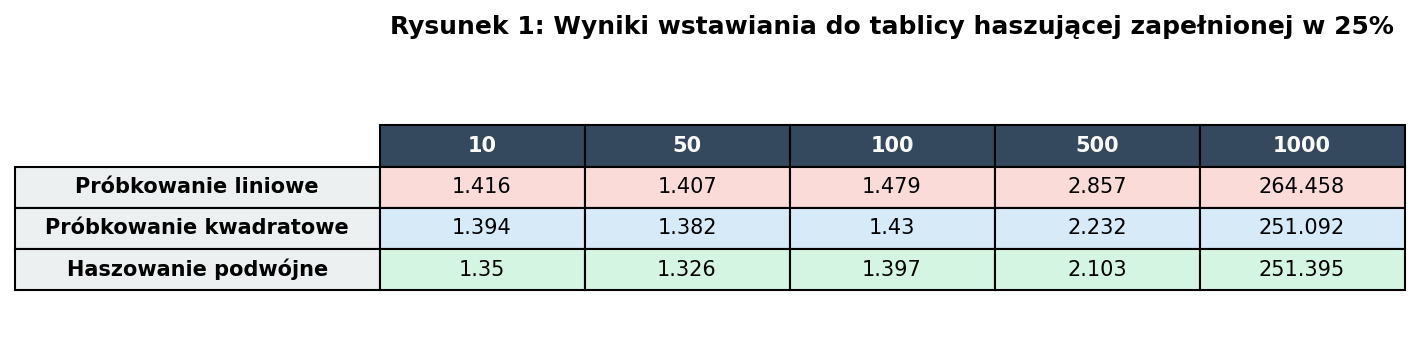
\includegraphics[width=0.8\textwidth]{wykresy/rys1_tablica_insert_25.png}
    \caption{Tablica przedstawiająca wyniki dla wstawiania danych do tablicy haszującej zapełnionej w 25\%}
\end{figure}

\begin{figure}[H]
    \centering
    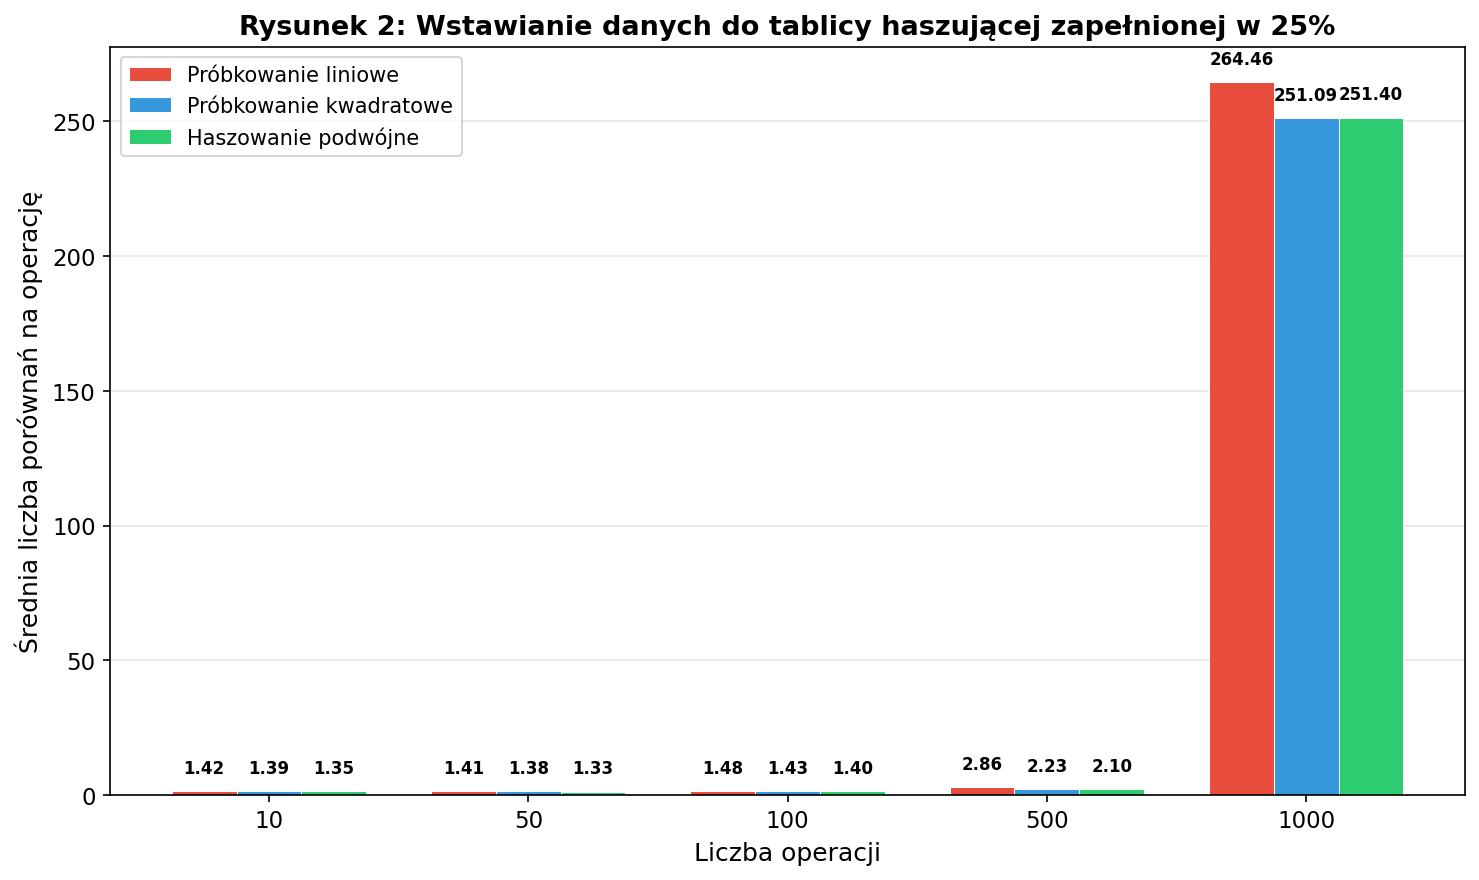
\includegraphics[width=0.8\textwidth]{wykresy/rys2_wykres_insert_25.png}
    \caption{Wykres dla wstawiania danych do tablicy haszującej zapełnionej w 25\%}
\end{figure}

Przy zapełnieniu rzędu 25\% kolizje występują rzadko. Próbkowanie liniowe, kwadratowe i haszowanie podwójne charakteryzują się bardzo niską liczbą porównań (bliską 1-1.5 na operację). Różnice między algorytmami są na tym etapie niemal niezauważalne, ponieważ tablica posiada mnóstwo wolnych miejsc.

% 50%
\begin{figure}[H]
    \centering
    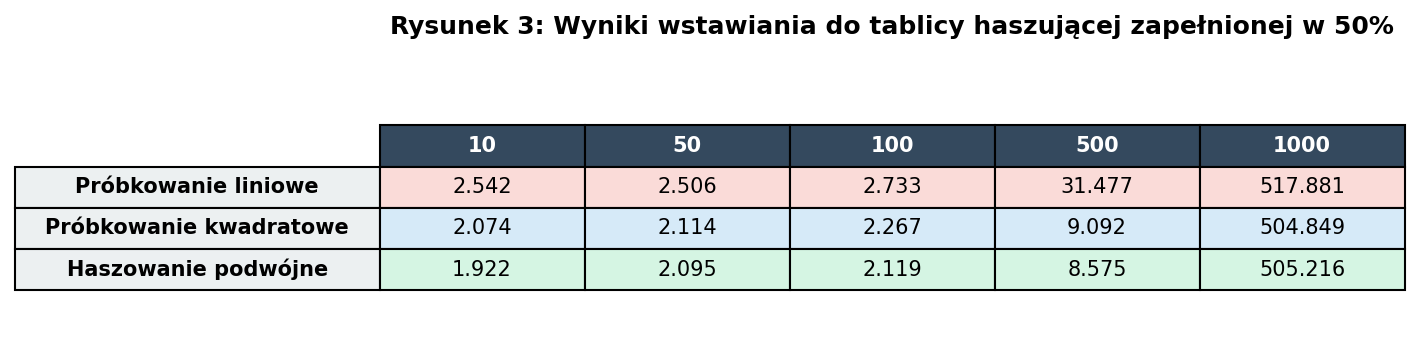
\includegraphics[width=0.8\textwidth]{wykresy/rys3_tablica_insert_50.png}
    \caption{Tablica przedstawiająca wyniki dla wstawiania danych do tablicy haszującej zapełnionej w 50\%}
\end{figure}

\begin{figure}[H]
    \centering
    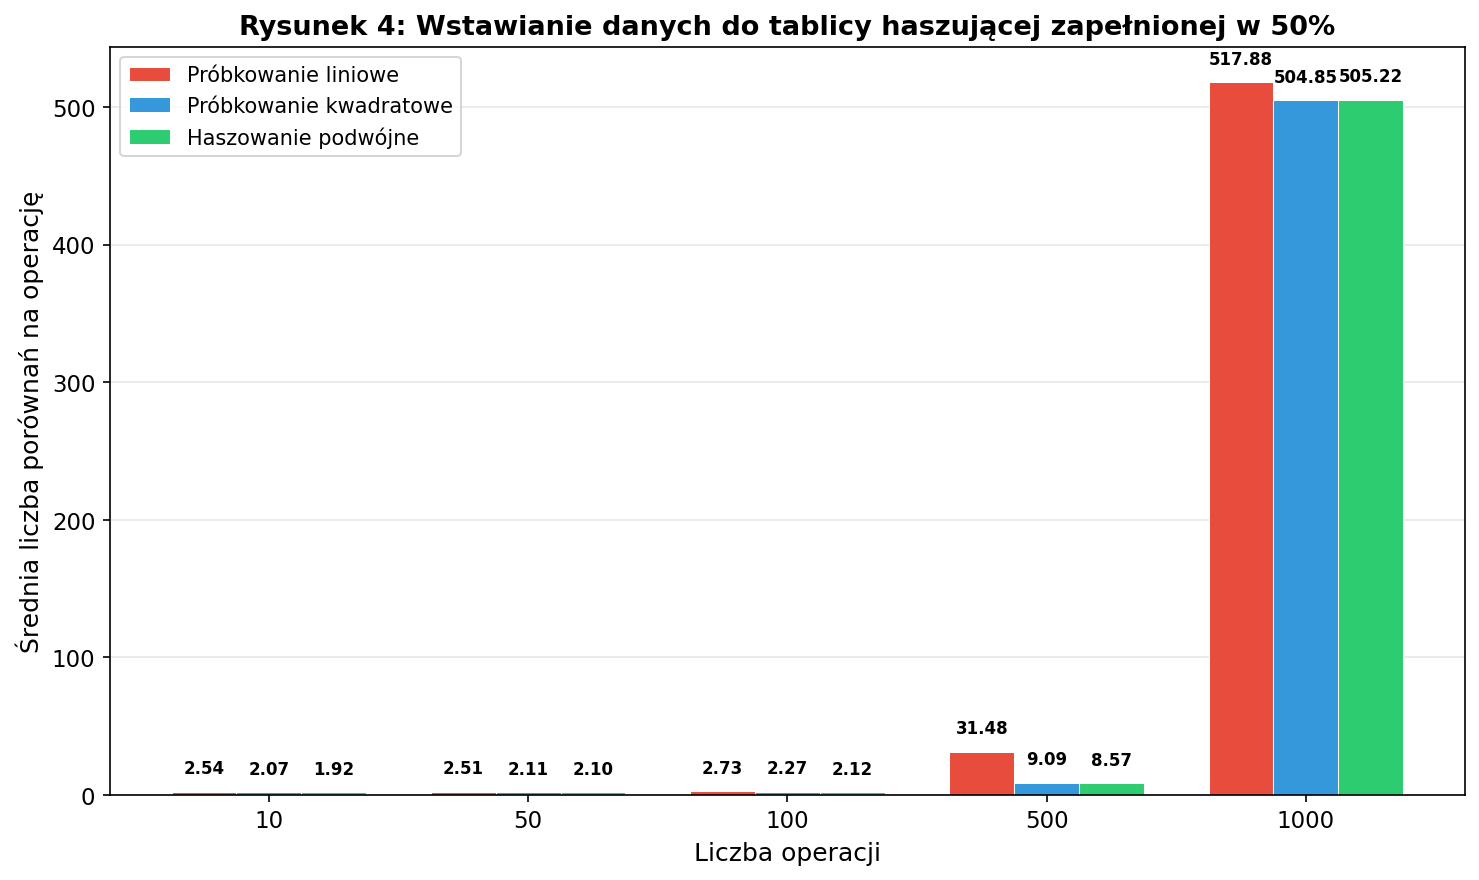
\includegraphics[width=0.8\textwidth]{wykresy/rys4_wykres_insert_50.png}
    \caption{Wykres dla wstawiania danych do tablicy haszującej zapełnionej w 50\%}
\end{figure}

Zapełnienie 50\% ukazuje pierwsze słabości próbkowania liniowego. Tworzące się tzw. klastry pierwotne zaczynają powoli degradować wydajność, zmuszając algorytm do sprawdzania coraz dłuższych ciągów zajętych komórek. Próbkowanie kwadratowe i haszowanie podwójne utrzymują przewagę i stabilność, skuteczniej omijając zagęszczone obszary.

% 75%
\begin{figure}[H]
    \centering
    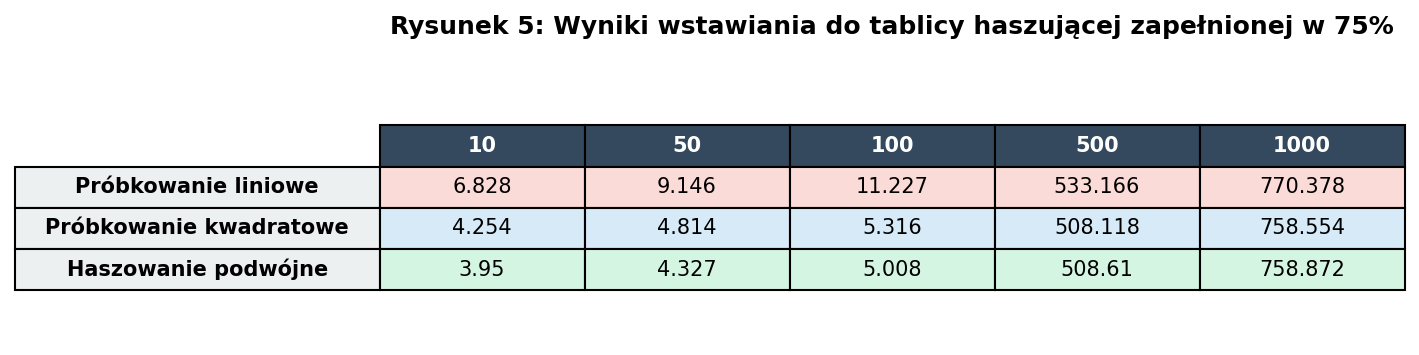
\includegraphics[width=0.8\textwidth]{wykresy/rys5_tablica_insert_75.png}
    \caption{Tablica przedstawiająca wyniki dla wstawiania danych do tablicy haszującej zapełnionej w 75\%}
\end{figure}

\begin{figure}[H]
    \centering
    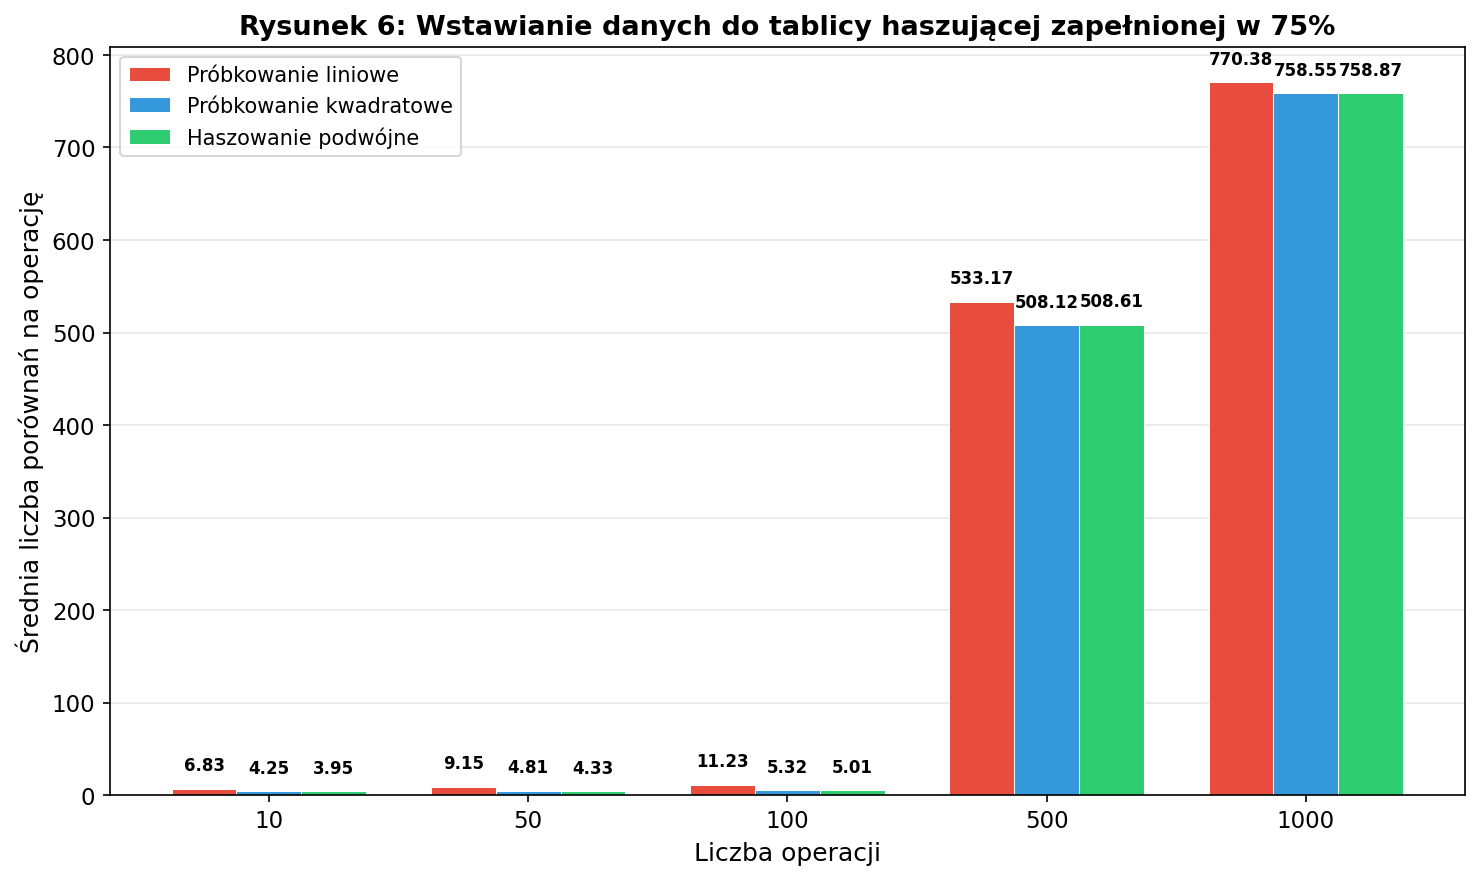
\includegraphics[width=0.8\textwidth]{wykresy/rys6_wykres_insert_75.png}
    \caption{Wykres dla wstawiania danych do tablicy haszującej zapełnionej w 75\%}
\end{figure}

Gdy zajętość tablicy osiąga 75\%, różnice stają się drastyczne. Próbkowanie liniowe odnotowuje olbrzymi skok liczby średnich porównań - dodawanie nowych elementów staje się bardzo kosztowne (wydajność drastycznie spada). Haszowanie podwójne wciąż radzi sobie zdecydowanie najlepiej, a próbkowanie kwadratowe wykazuje umiarkowane pogorszenie wyników ze względu na zjawisko klastrowania wtórnego.

\subsection{Badanie usuwania z tablicy haszującej}
W przypadku adresowania otwartego usuwanie (Delete) opiera się najczęściej o technikę wstawiania specjalnych znaczników (tzw. "Tombstones" lub węzłów oznaczonych jako USUNIĘTE). W badaniach zliczono ilość próbkowania potrzebną do odnalezienia usuwanego klucza. Zjawiska spadku wydajności są tutaj analogiczne do operacji wstawiania, gdyż do usunięcia elementu niezbędne jest jego uprzednie wyszukanie.

% 25%
\begin{figure}[H]
    \centering
    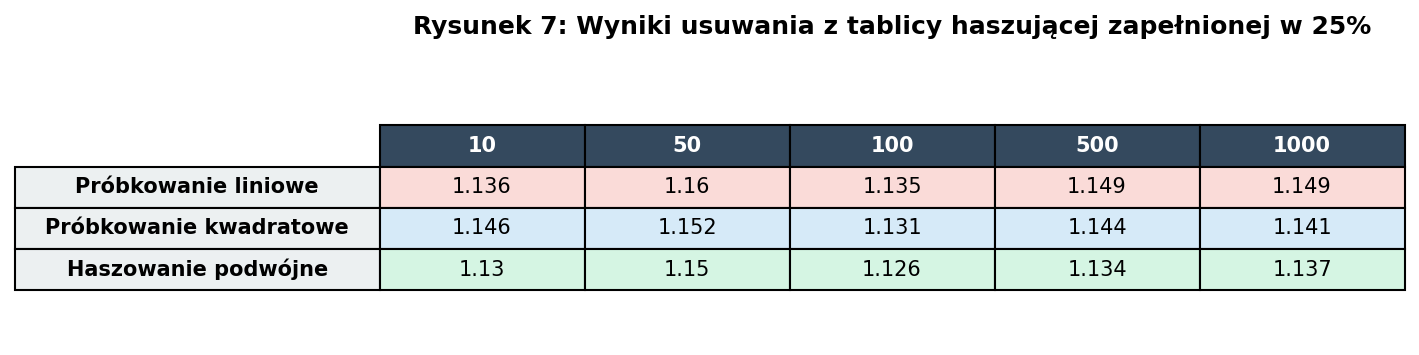
\includegraphics[width=0.8\textwidth]{wykresy/rys7_tablica_delete_25.png}
    \caption{Tablica przedstawiająca wyniki dla usuwania danych z tablicy haszującej zapełnionej w 25\%}
\end{figure}

\begin{figure}[H]
    \centering
    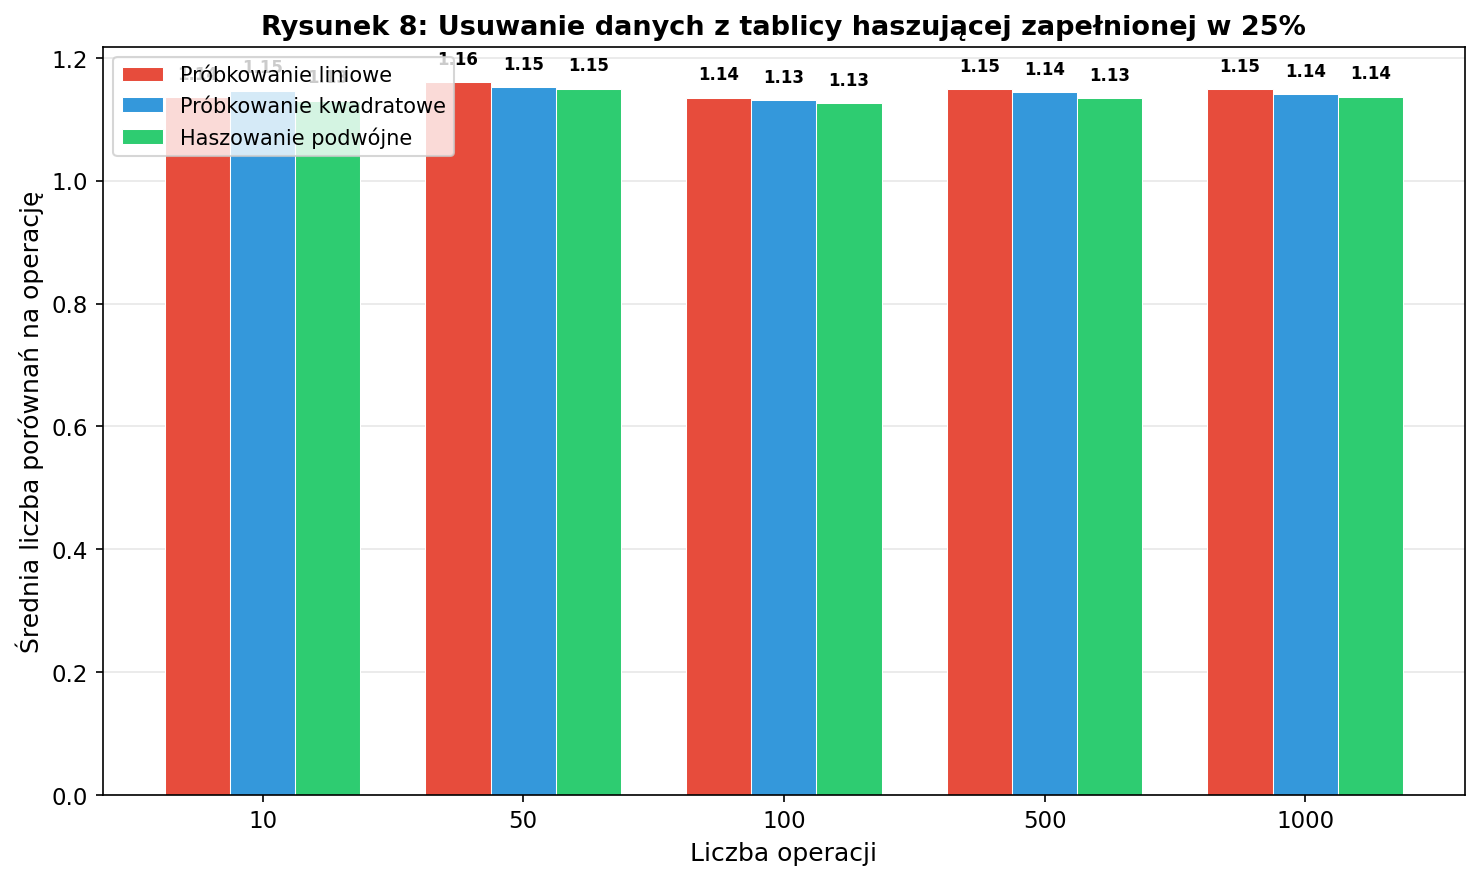
\includegraphics[width=0.8\textwidth]{wykresy/rys8_wykres_delete_25.png}
    \caption{Wykres dla usuwania danych z tablicy haszującej zapełnionej w 25\%}
\end{figure}

W luźno wypełnionej tablicy (25\%) usunięcie danych wymaga sprawdzenia niewiele więcej niż jednej komórki, niezależnie od zastosowanej metody. Odnalezienie elementu jest błyskawiczne ze względu na brak długich łańcuchów kolizji.

% 50%
\begin{figure}[H]
    \centering
    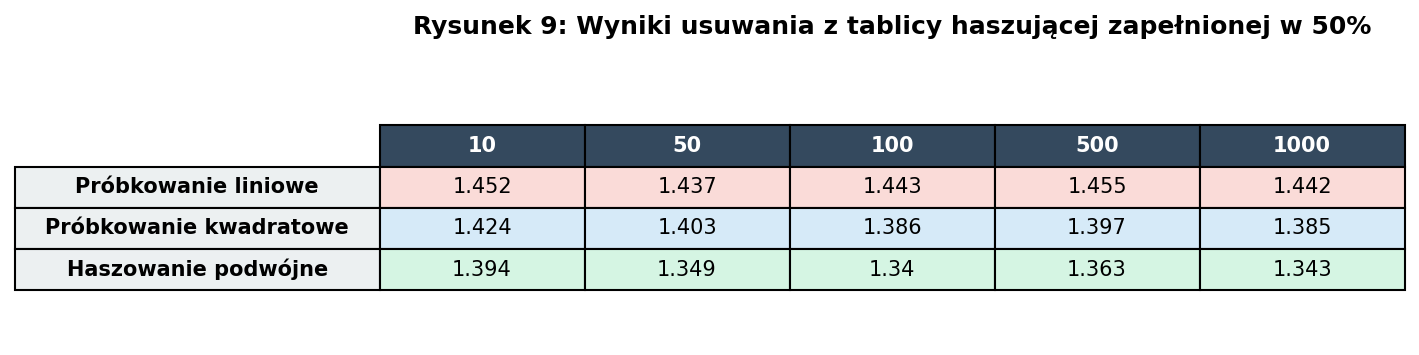
\includegraphics[width=0.8\textwidth]{wykresy/rys9_tablica_delete_50.png}
    \caption{Tablica przedstawiająca wyniki dla usuwania danych z tablicy haszującej zapełnionej w 50\%}
\end{figure}

\begin{figure}[H]
    \centering
    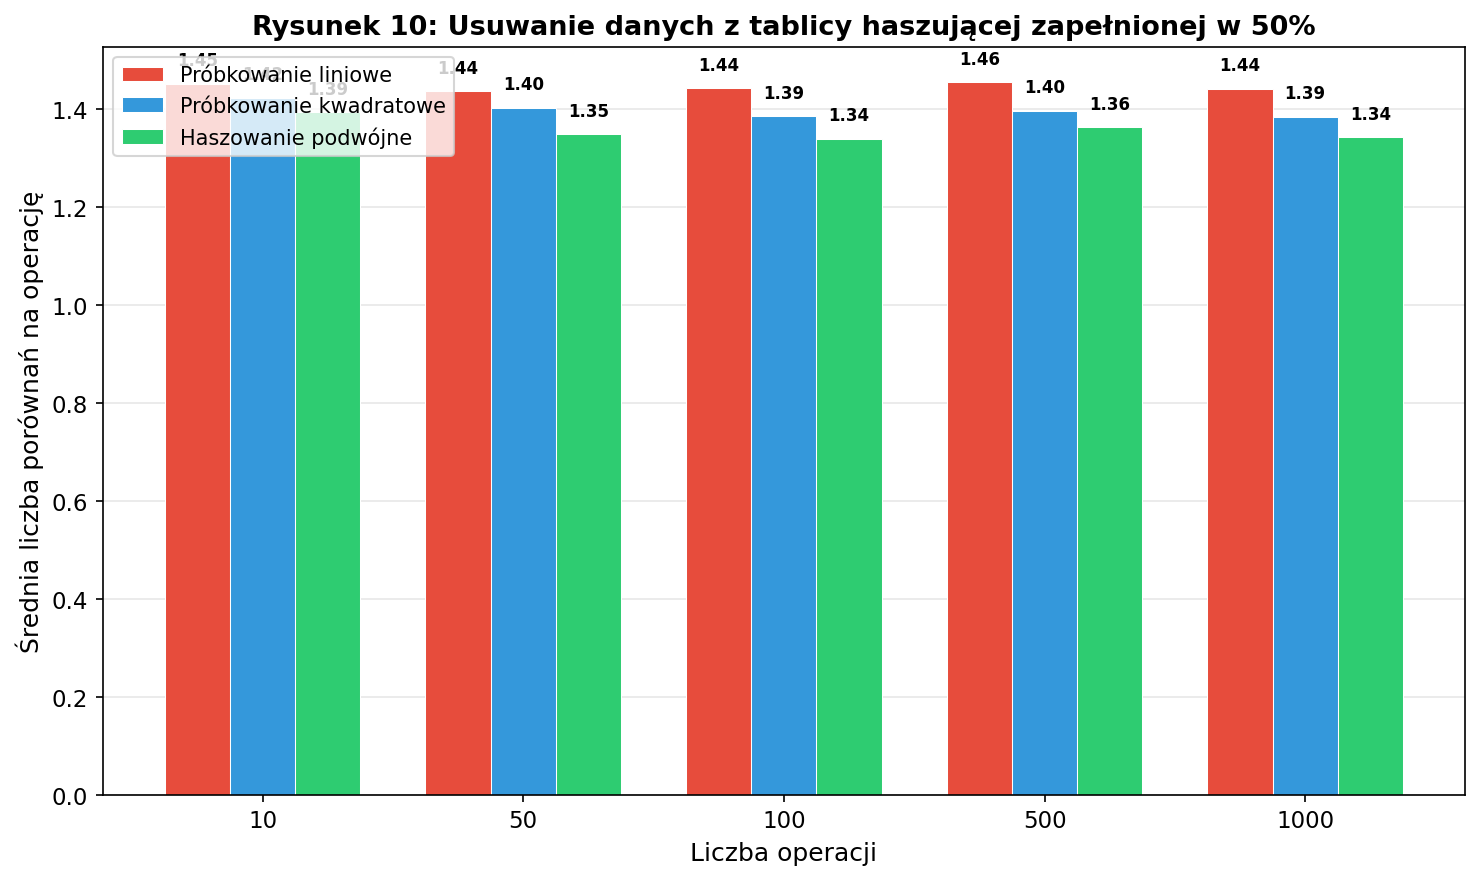
\includegraphics[width=0.8\textwidth]{wykresy/rys10_wykres_delete_50.png}
    \caption{Wykres dla usuwania danych z tablicy haszującej zapełnionej w 50\%}
\end{figure}

Przy 50\% wypełnieniu proces przeszukiwania dla adresowania liniowego zaczyna spowalniać. Klastry zbudowane podczas wstawiania stają się na tyle długie, że wyszukiwanie elementów wymaga kilkukrotnego odpytania tablicy. Wypadkowo lepiej radzi sobie tu podwójne haszowanie, gdzie rozstrzelenie elementów gwarantuje szybsze dotarcie do szukanego klucza.

% 75%
\begin{figure}[H]
    \centering
    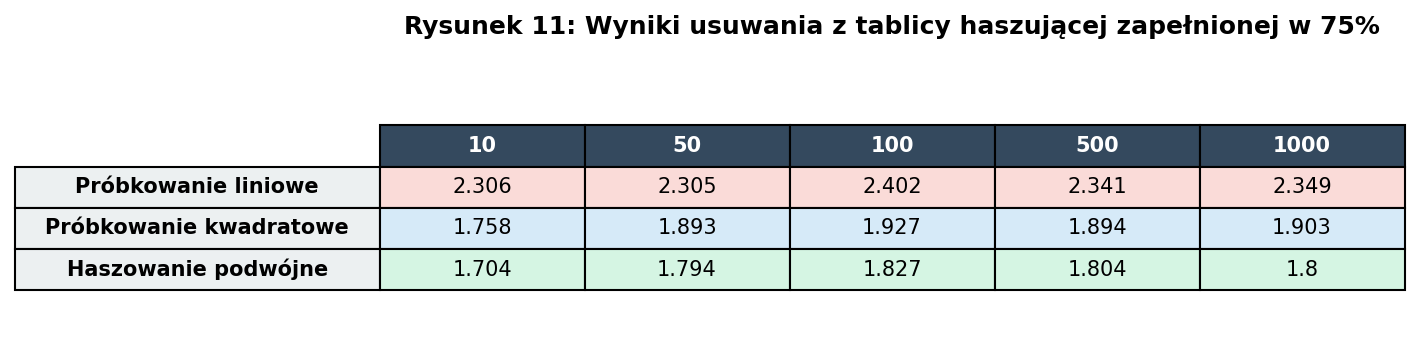
\includegraphics[width=0.8\textwidth]{wykresy/rys11_tablica_delete_75.png}
    \caption{Tablica przedstawiająca wyniki dla usuwania danych z tablicy haszującej zapełnionej w 75\%}
\end{figure}

\begin{figure}[H]
    \centering
    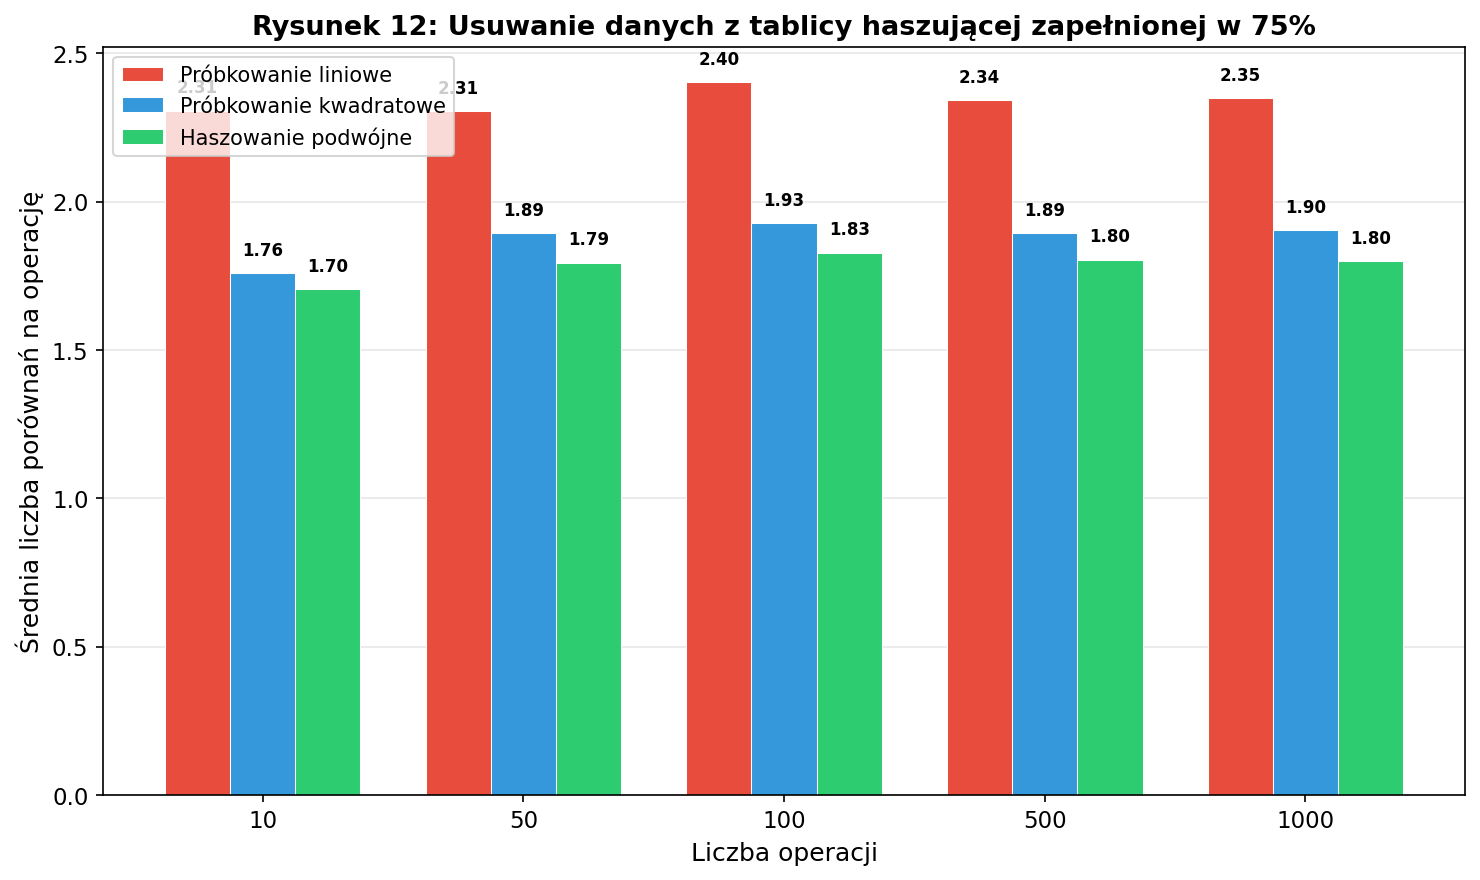
\includegraphics[width=0.8\textwidth]{wykresy/rys12_wykres_delete_75.png}
    \caption{Wykres dla usuwania danych z tablicy haszującej zapełnionej w 75\%}
\end{figure}

Najwyższe zaprezentowane zapełnienie (75\%) jednoznacznie potwierdza ułomność próbkowania liniowego. Znalezienie węzła do usunięcia wymaga liniowego przejścia przez spory blok zbitych ze sobą komórek. Próbkowanie kwadratowe wypada znacznie lepiej, natomiast absolutnym zwycięzcą okazuje się haszowanie podwójne, wymagające najmniejszej liczby porównań w celu zlokalizowania odpowiedniego wpisu.

\section{Wnioski}
Przeprowadzone badania i analiza wybranych metod rozwiązywania kolizji pozwalają na wyciągnięcie następujących wniosków:
\begin{enumerate}
    \item \textbf{Wpływ stopnia zapełnienia (\textit{load factor}):} Stopień wypełnienia tablicy haszującej jest krytycznym parametrem wpływającym na wydajność. O ile dla wartości rzędu 25\% każda z metod radzi sobie doskonale w czasie stałym $O(1)$, o tyle przekroczenie poziomu 50-70\% dramatycznie pogarsza charakterystyki czasowe niektórych algorytmów. 
    \item \textbf{Problemy adresowania liniowego:} Próbkowanie liniowe to podejście najprostsze w implementacji, ale bardzo wrażliwe na powstawanie klastrów pierwotnych. Zlepianie się wielu kluczy w ciągłe bloki potęguje ilość kolizji dla kolejnych elementów.
    \item \textbf{Przewaga haszowania podwójnego:} Haszowanie podwójne charakteryzuje się najrówniejszym rozkładem i najniższą degradacją w czasie. Dzięki wykorzystaniu dodatkowej funkcji haszującej do określenia kroku, unika ono zarówno klastrowania pierwotnego, jak i wtórnego, co było wyraźnie widać w próbach wstawiania i usuwania przy 75\% zapełnieniu.
    \item \textbf{Nowoczesne podejścia:} Rozwiązania w stylu \textit{Robin Hood hashing} oraz \textit{Cuckoo hashing} stanowią potężną alternatywę tam, gdzie klasyczne próbkowanie nie wystarcza. Gwarantują one odpowiednio stałe limity najgorszego przypadku lub niwelują wariancję czasów operacji.
\end{enumerate}

W praktyce dobór strategii zarządzania kolizjami zawsze stanowi kompromis pomiędzy stopniem skomplikowania kodu a wymaganą optymalizacją. Tablice z adresowaniem liniowym wymagają bardzo restrykcyjnego powiększania rozmiaru (\textit{rehashing}) dużo wcześniej (często już przy $\approx 50\%$ zapełnienia), podczas gdy zaawansowane metody jak kukułcze czy Robin Hood pozwalają utrzymywać stabilność operacyjną do wyższych wartości \textit{load factor} bez utraty stałego czasu wyszukiwania.

\end{document}
